\documentclass[dvipdfmx,autodetect-engine,titlepage]{jsarticle}
\usepackage[dvipdfm]{graphicx}
\usepackage{ascmac}
\usepackage{fancybox}
\usepackage{listings}
\usepackage{plistings}
\usepackage{itembkbx}
\usepackage{amsmath}
\usepackage{svg}
\usepackage{url}
\usepackage{graphics}
\usepackage{listings,jvlisting}

\textheight=23cm
\renewcommand{\figurename}{図}
\renewcommand{\tablename}{表}
\newenvironment{code}
{\vspace{0.5zw}\VerbatimEnvironment  \begin{screen} 
\baselineskip=1.0\normalbaselineskip
 \begin{Verbatim}}
{\end{Verbatim}
\baselineskip=\normalbaselineskip
 \end{screen}\vspace{0.5zw}} 

\title{情報理工学部 SNコース 2回\\
セキュリティ・ネットワーク学実験2\\
課題6-2レポート}
\author{2600200443-6\\Yamashita Kyohei\\山下 恭平}
\date{November 5 2021}

\begin{document}

\maketitle

\section{概要}
近距離無線 Bluetooth Low Energy(BLE)を用いて、スマートフォンとRaspberry
Piとの間で通信を行うことを目的とする実験。

\section{実験概要}

\subsection{実験で使用した機材}
今回の実験では、Raspberry Piとアンドロイドスマートフォンを使用した。以下の
図はそれら写真である。

\begin{figure}[h]
  \centering
  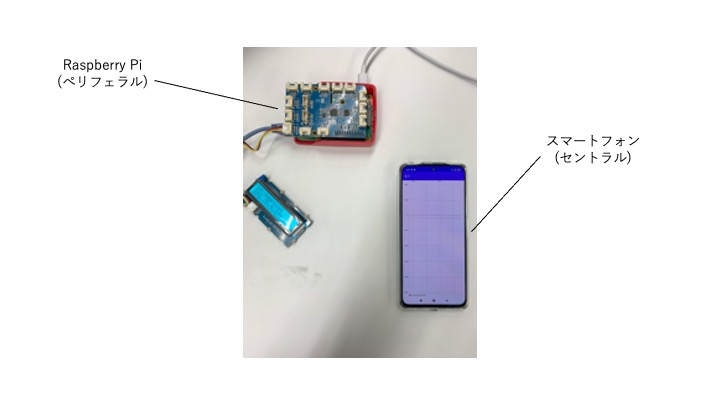
\includegraphics[scale=0.4]{pic1.JPG}
  \caption{機材の写真}
\end{figure}

\subsection{実験の様子}
Raspberry Piから広告パケットを送信し続け、スマトーフォンで受信する。初めは、
至近距離から広告パケットを受け取り、徐々に距離を離していきながら、受信強度を測定
した。距離の測定方法として、実験室の床のタイル1枚を50cmとして測定した。

\begin{figure}[h]
  \centering
  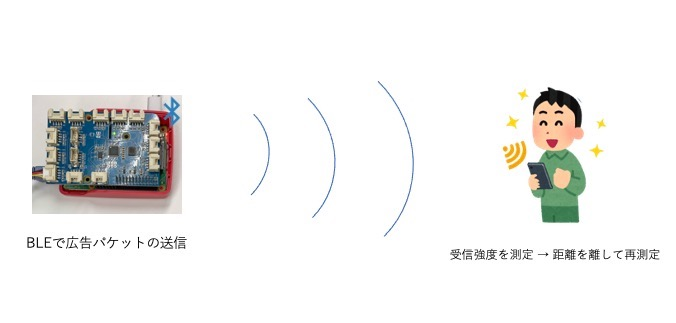
\includegraphics[scale=0.4]{pic2.jpg}
  \caption{実験様子のイラスト}
\end{figure}

\subsection{実験の手順}
Raspberry Piから広告パケットを送信し続け、スマトーフォンで受信する。初めは、
至近距離から広告パケットを受け取り、徐々に距離を離していきながら、受信強度を測定
した。距離の測定方法として、実験室の床のタイル1枚を50cmとして測定した。

\section{実験結果}
実際に測定した結果は以下の写真である。

\begin{figure}[h]
  \centering
  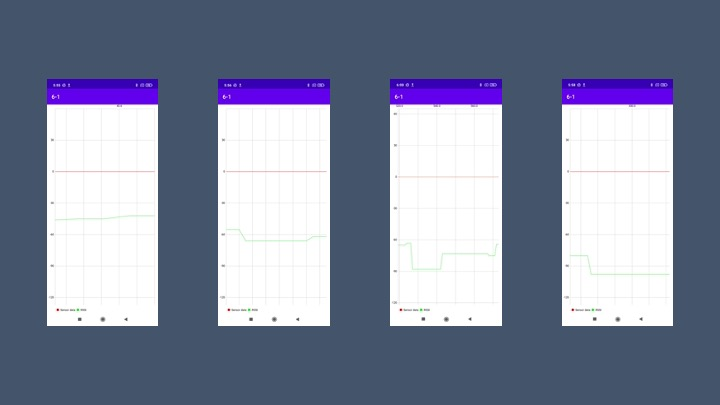
\includegraphics[scale=0.3]{pic4.jpg}
  \caption{測定結果 1}
\end{figure}

次の表は、測定したデータをまとめたものである。

\begin{table}[h]
  \centering
  \caption{測定結果 2}
  \begin{tabular}{|l||l|l|l|l|l|}
  \hline
  距離   & 0m  & 2.5m & 5m  & 7.5m & 10m  \\ \hline
  RSSI & -45 & -65  & -80 & -90  & -100 \\ \hline
  \end{tabular}
  \end{table}

  表をもとに、グラフを作成し、近侍直線を引いたものが以下の図である。 \\

\begin{figure}[h]
  \centering
  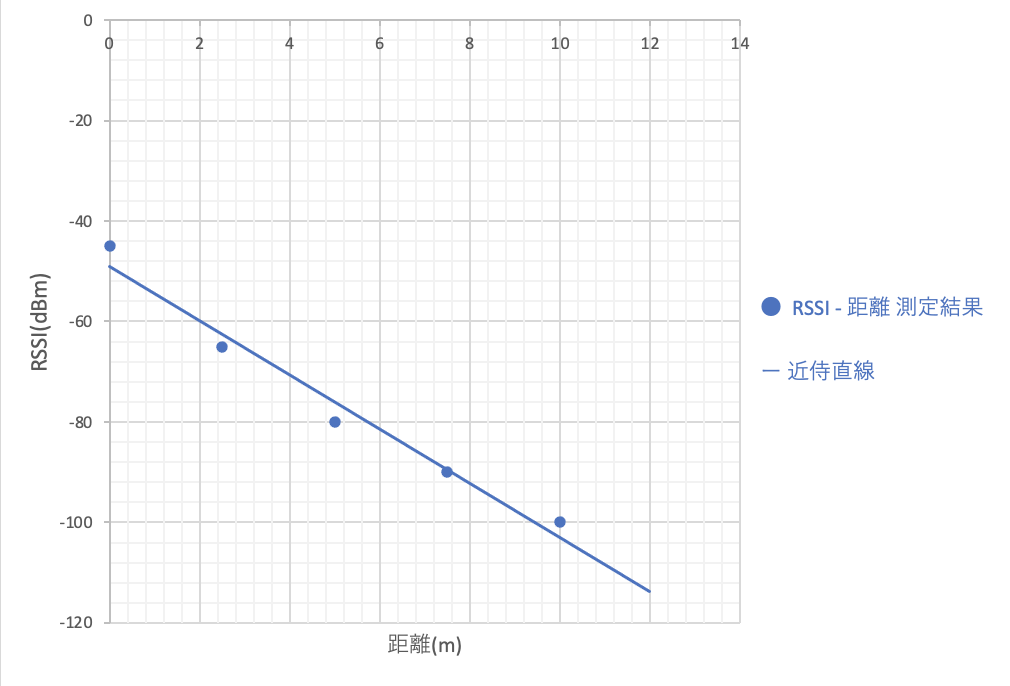
\includegraphics[scale=0.5]{pic3.png}
  \caption{距離とRSSIの関係}
\end{figure}

以下の図は教室の端から、自分の席に向かってゆっくり近づいて行った時の測定結果である。\\

\begin{figure}[h]
  \centering
  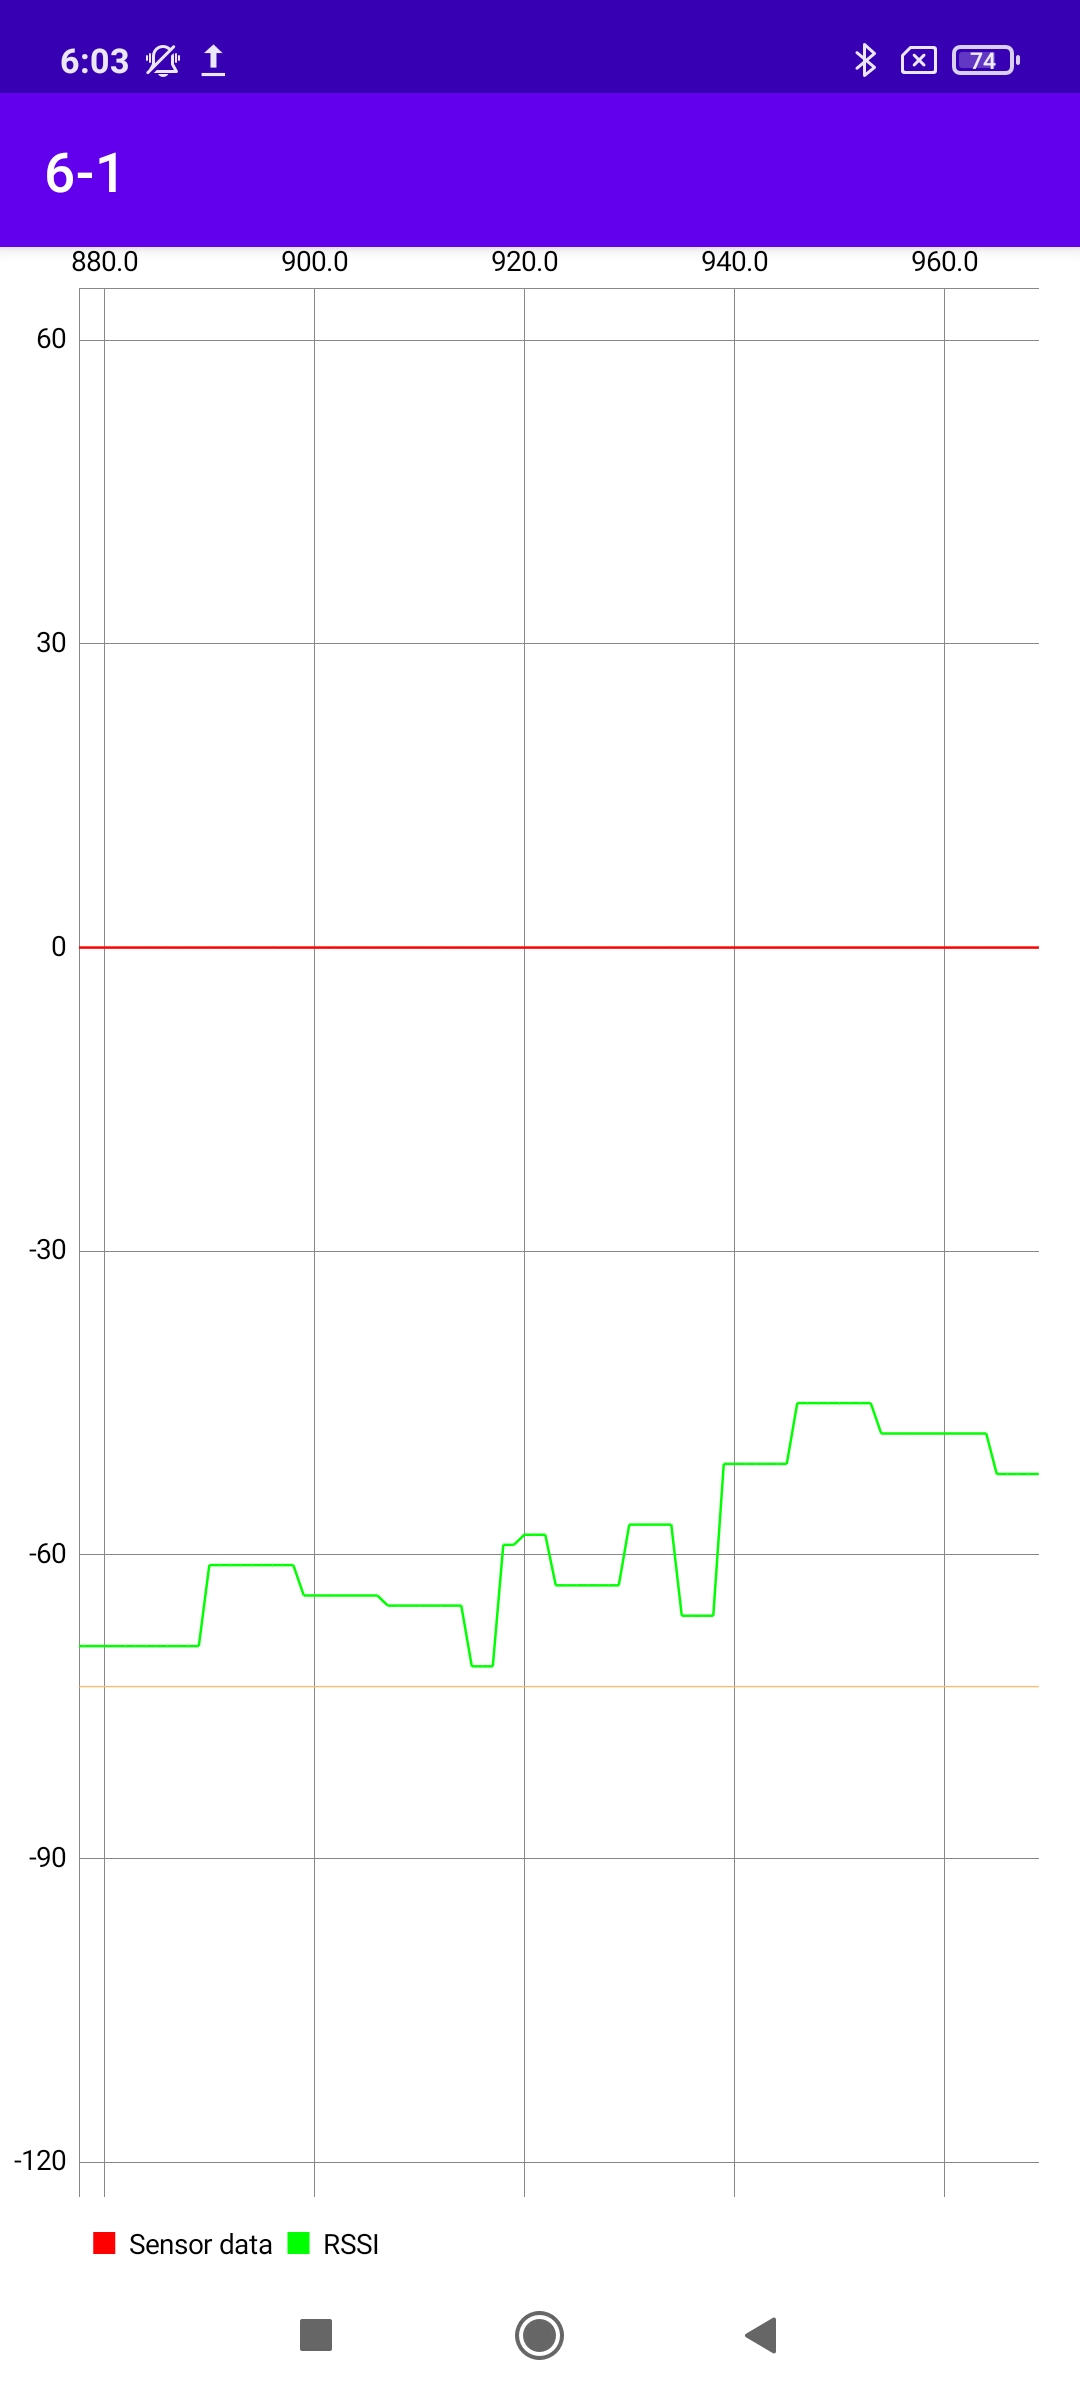
\includegraphics[scale=0.1]{pic5.jpg}
  \caption{測定結果}
\end{figure}

\section{考察}
今回の測定結果は、複数回実験を行った中で最も綺麗に値が収集できたものを使用した。
繰り返し測定を行った結果、値の大きさは教室の混雑状況などにより異なったが、距離が遠ざかる
につれて、値が小さくなっていくことについては一致した。また、図5の測定結果は、教室の端から自席
まで歩いて測定を行ったものであるが、近づくにつれて値が回復していることがわかる。また、
図4の近似直線より、RSSIと距離は比例していることが読み取れる。よって、BLEは室内などの
限られたエリアでの位置情報サービスにおいては利用可能だと考えられる。

\end{document}